\documentclass[12pt]{amsart}
\usepackage{../marktext} 
%% Remove draft for real article, put twocolumn for two columns
\usepackage{../svmacro}
\usepackage[utf8]{inputenc}
\usepackage{lineno}
%\usepackage{authblk}
\usepackage[style=alphabetic, backend=biber]{biblatex}
\usepackage{enumitem}

%% commentary bubble
\newcommand{\SV}[2][]{\sidenote[colback=green!10]{\textbf{SV\xspace #1:} #2}}

%% Title 
\title{ MATH 170: Homework 7 }
%\author[1]{Co-author}
\author{Due: Nov 12, 2021}
%\affil[1]{Institute}
\date{}

\begin{document}

\maketitle


\noindent{\bf Graded for accuracy:}
1,2.
\\
\noindent{\bf Graded for completion:}
\\
\noindent{\bf Instructions:}
Problems that are graded for accuracy must be correct to get points.
Problems that are graded for completion must show some trying effort.

\centerline

\hrule

\centerline

\begin{enumerate}[label=\arabic*.,itemsep=10pt, leftmargin=*]


    \item 
        \begin{enumerate}
            \item 
        Draw the following graph $G = (V,E)$ where
        \begin{equation*}
            V = \set{ a,b,c,d,e,f,g}
        \end{equation*}
        and 
        \begin{equation*}
            E = \set{ab, aa, ad,af, be,eb, de,ed, ef, fa, fd, ff, cg } \,.
        \end{equation*}

        \item Is $G$ connected?
        \item If it is not connected, how can you fix it so that it is connected?
            Write down using mathematical symbols as in part (a) to represent
            the new graph you found.
        \item Is there an Eulerian path through your graph?
        \item Is there an Eulerian cycle through your graph?
        \end{enumerate}
    
\item Island Linear has 10 countries on it, the map looks like this:
\begin{center}
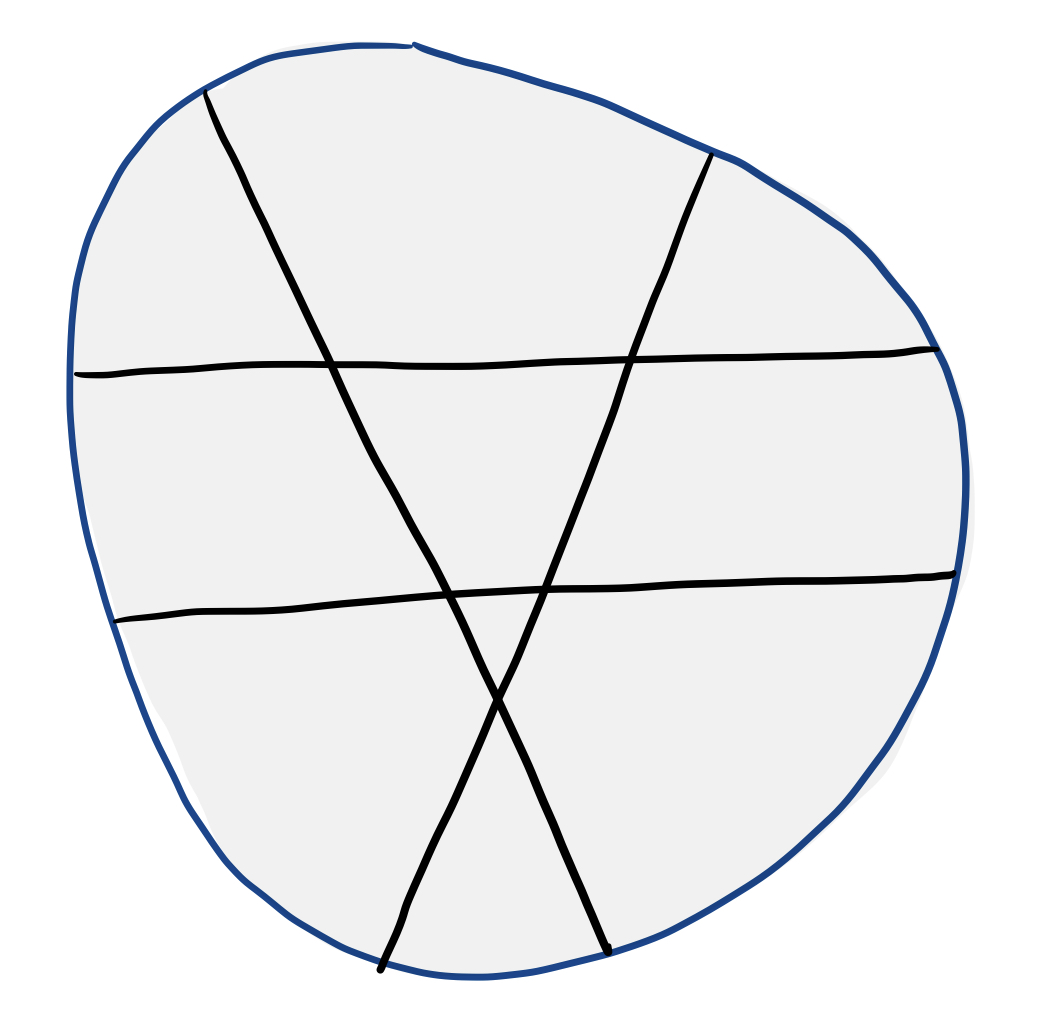
\includegraphics[width=7cm,height=5cm]{IMG_7163.jpg}
\end{center}
    \begin{enumerate}
        \item Draw the graph dual to this map.
        \item Can you color this graph in two colors such that vertices of the same color never share an edge?
        \item What is the chromatic number of this graph?
    \end{enumerate}
\end{enumerate}



\end{document}
